\subsection{Summary of the Exoplanet Catalog}

The final DR25 KOI catalog, available at NExScI contains all of the planet candidates and all TCEs that did not fail due to one of the not-transit like tests (\S\ref{nottransitlikesec}). 


Some overall statistics of the DR25 KOI catalog are as follows:
\begin{itemize}
    \item 8054~KOIs
    \item 4034~Candidates
    \item XXXX new KOIs
    \item XX210XX new Candidates
    \item 85 per cent overall completeness
    \item 97 per cent overall reliability
\end{itemize}

A summary of the planet radii and period of the planet candidates available in this catalog can be seen in Figure~\ref{f:catalogPlot}. The deficit of planets with radii near 2.0\,R$_{\oplus}$ is consistent with the study of \citet{Fulton2017} where they report a natural gap in the abundance of planets between super-Earths and sub-Neptunes by applying precise stellar parameters to a subset of the \kepler\ transiting candidates. A clear excess of candidates exists for PCs with periods near to 370\,d;  with a score cut of $\approx0.8$, this excess disappears. While the disposition score provides an easy way to make an additional cut on the PC population at long periods, when discussing the catalog PCs below we are using the pure dispositions of the Robovetter unless otherwise stated. 

The new KOIs with a disposition of PC are found at all periods. The overwhelming majority of these new PCs have MES less than 9.  Only 10XX have MES >= 10, and just 3XX of these have MES > 12. 

\begin{figure*}
    \centering
    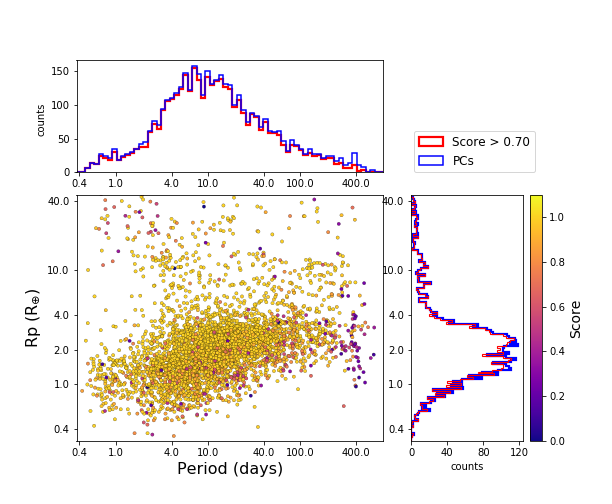
\includegraphics[width=1.1\linewidth]{fig-radiusPeriodScore-hist.png}
    \caption{DR25 planet candidates plotted as planet radius against Period with the color representing the disposition score. Those plotted in orange and yellow are those whose metrics lie near to the lest confident PCs.  The period and planet radii distributions are plotted on the top and on the left, respectively, in blue. The red line shows the distributions if you only consider those KOIs with a score greater than 0.8. }
    \label{f:catalogPlot}
\end{figure*}





%\subsection{Comparison to Previous KOI Catalogs}

\subsection{Comparison to Confirmed Exoplanets}
There are two set of \Kepelr\ exoplanets that have been thoroughly vetted by hand, the confirmed exoplanets and the certified false positives.  In both of these cases that utilize additional observations to fully validate the signal as either an exoplanet or a False Positive.  It is worth comparing the Robovetter to these data as a sanity check.  We pulled the Kepler Confirmed planets from NExScI

\subsection{Comparison to the FPWG false positives}



%MUCH IS MISSING, HERE ARE SOME IDEAS:
%\begin{itemize}
%    \item [o] plot of pradius vs. period and/or pradius vs insol. flux
%    \item [o] Histogram of number of candidates of different sizes (short and long period)
%    \item [o] Discuss number of candidates compared to previous catalogs.
%    \item [o] Discuss identified EBs.
%    \item [o] From looking at distributions obvious over abundance at 370 days.
%\end{itemize}